\chapter{Simulation}
\label{Sim}
Network simulation is a practical way of developing and researching networks and their
behaviors. Especially in WSNs, the main focus is not on one particular sensor node, but on
the behavior of the entire network (which can consist of thousands of sensor nodes). It would
be impractical to do initial research based on real world testing and deployment, as that would cost exorbitant amounts of money, and create logistical nightmares in the WSN setup. For this reason a valid
simulation tool is a necessity for further studies. This chapter focuses on the simulation; it 
includes discussion about the simulator, simulation execution, scenario setups and simulation procedure.

\section{TinyOS Simulator - TOSSIM}
\label{Sim:TOSSIM}

The simulator used in this project is called TOSSIM\@. TOSSIM is a discrete, event-driven WSN simulator included in TinyOS. Compiling unchanged TinyOS applications
directly into its framework, TOSSIM can simulate thousands of motes running complete
applications~\cite{LLWC}. It fulfils the requirements of being a TinyOS simulator; such requirements include: scalability, completeness and fidelity. TOSSIM is a shared library, therefore a script written with C++ or Python must be created to run the simulation.  Python is chosen in this thesis as it can dynamically interact with the simulation.

Configuring networks for TOSSIM simulation usually includes setting
up a network topology and an interference model. For the topology, a file with the format~\texttt{Source Destination Gain} needs to be created. TOSSIM uses the Closest Pattern Matching (CPM) algorithm to calculate channel noise. It is a wireless noise simulation model
based on statistical extraction from empirical noise data. It works by taking a noise trace as input to generate the interference model. This method is accepted to be much more accurate and preferable than the traditional, Independent Packet Loss (IPL) models~\cite{TOSSIM}.

\section{Enabling the Simulation}
\label{Sim:Enabling}

The simulation had already been enabled for a multi-hop network using the BLIP 1.0 implementation before. The radio stack for this simulation was the CC2420. But due to the significant changes that were done to both the CC2420 radio stack and BLIP, considerable work was required to re-enable the simulation of BLIP 2.0. 

As mentioned in Section~\ref{Sim:radio stack}, the rfxlink radio stack unifies CC2420 and RF230. Furthermore, the TOSSIM simulation support for rfxlink has been developed by Morten Tranberg Hansen~\cite{rfxsim}. But neither BLIP 1.0 nor BLIP 2.0 have been implemented on top of rfxlink. In oder to execute the simulation, the simulated rfxlink had to be moved underneath BLIP 2.0. 

The re-enabling of the simulation required the following steps: 
\begin{itemize}
\item Merging of the branch of Morten Tranberg Hansen's rfxsim repository~\cite{rfxsim}. 

\item Adding the simulated ``chip driver'' layer - TossimDriverLayerC to the already supported CC2420 and RF230 radio chips of rfxlink. 

\item Introducing 802.15.4 packets into TOSSIM. TinyOS basic packets abstraction is Active Message (AM), but 6LoWPAN uses 802.15.4 packets. Introduction of 802.15.4 packets into TOSSIM is essential for the simulation to run.

\item Configuring the simulation to support BLIP 2.0. Using short IEEE 802.15.4 addresses for \texttt{Ieee154Send} interface in the component \texttt{IPDispatch}. 

\item The compiler GPP is used to compile BLIP 2.0, while the 6LoWPAN library is written in C. The \texttt{extern ``C''} had to be added to notify the C++ compiler of the C style functions.

\item A Makefile had to be written to include 6LoWPAN object files into the simulation library.
\end{itemize}

\section{Simulation Setups}
\label{Sim:Setup}
\subsection{Methodology}
\label{Sim:Method}
The application~\texttt{UDPEcho} is used in the simulation to evaluate the performance of the RPL protocol. It is configured to behave similarly to the application~\texttt{Ping}. A node sends out a data packet to another node, which replies back to the original sender. However, this is done on the application layer. The application is installed on the simulated root node and the child nodes. In the simulation, the root node will send 100 \texttt{UDPEcho} packets one after another to a child node, then continue to send another 100 \texttt{UDPEcho} packets to the next child node, until all child nodes are  ``pinged''.     

The simulation is done for various scenarios with different number of nodes, as well as with objective functions OF0 and MRHOF. The results of the simulation is visualized with the python plotting library~\texttt{Matplotlib}.

\subsection{Simulation Scenarios}
\label{Sim:Scenarios}

Two kinds of scenarios are created for the simulation - a line scenario and a grid scenario. In the line scenario the neighboring nodes are equally distanced; in the grid scenario, the number of nodes should be a square number, and the grids are square grids. Figure~\ref{fig:scenario_line} shows a 4-node line scenario with 10-meter inter-node distance. A 9-node grid scenario with 100-meter inter-node distance is shown in Figure~\ref{fig:scenario_grid}. Node 1 is configured to be the root node in the simulation.

\begin{figure}[htpb]
 % \begin{center}
 	\centering
    \leavevmode
    %\framebox{
      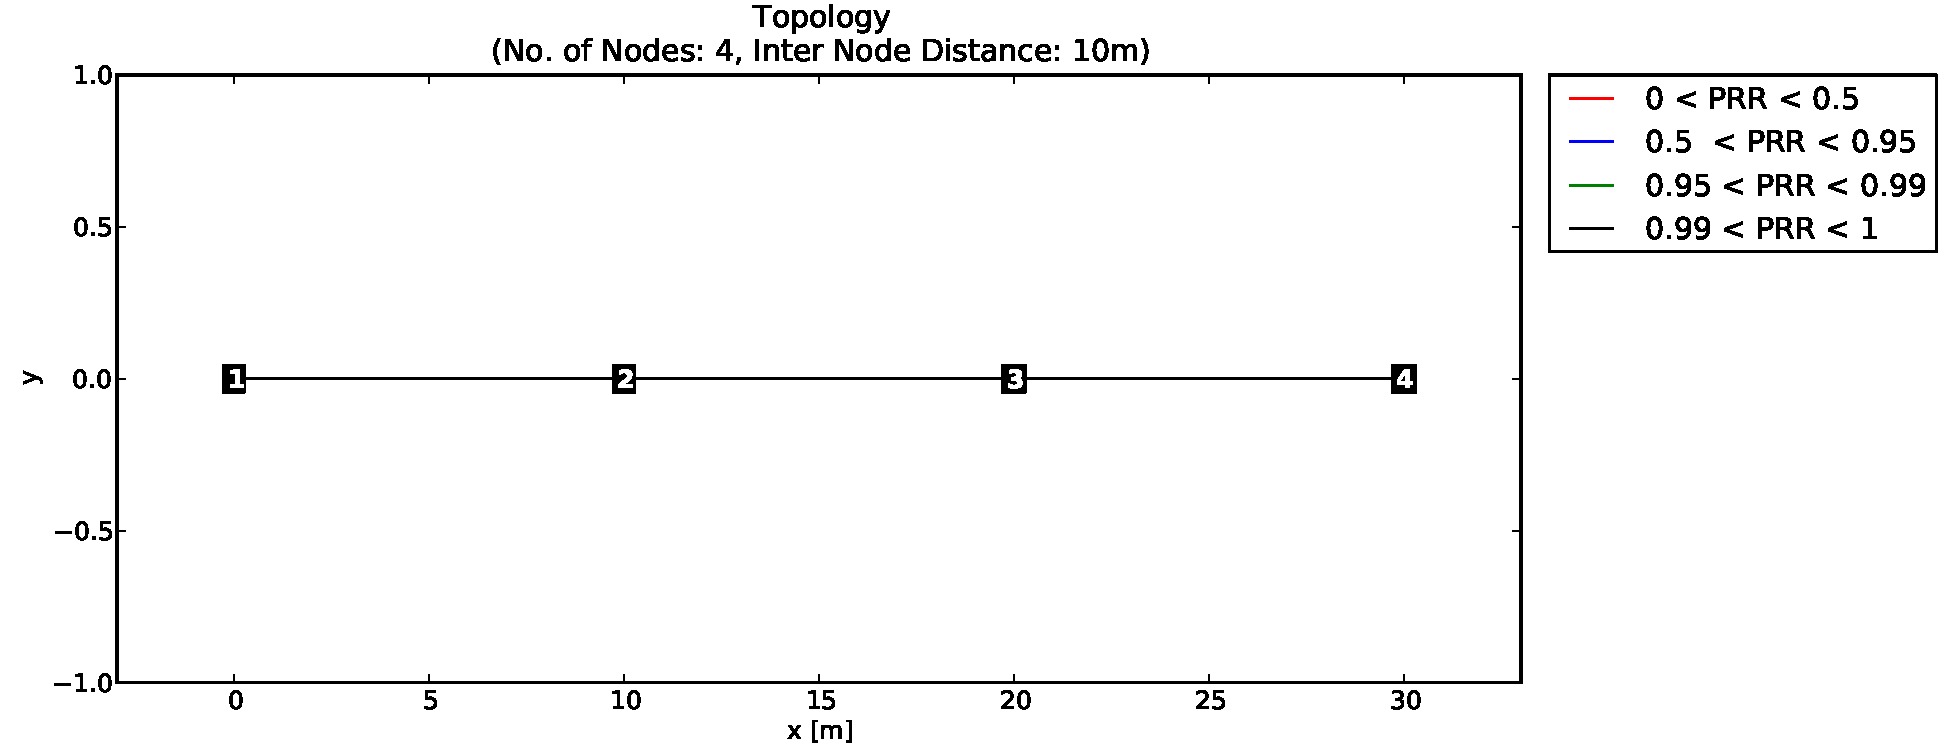
\includegraphics[scale=0.35]{Pics/results/topo4_dist10_line.pdf}
    \caption{Line scenario}
    \label{fig:scenario_line}
\end{figure}

\begin{figure}[htpb]	
%  \begin{center}
  	\centering
    \leavevmode
    %\framebox{
      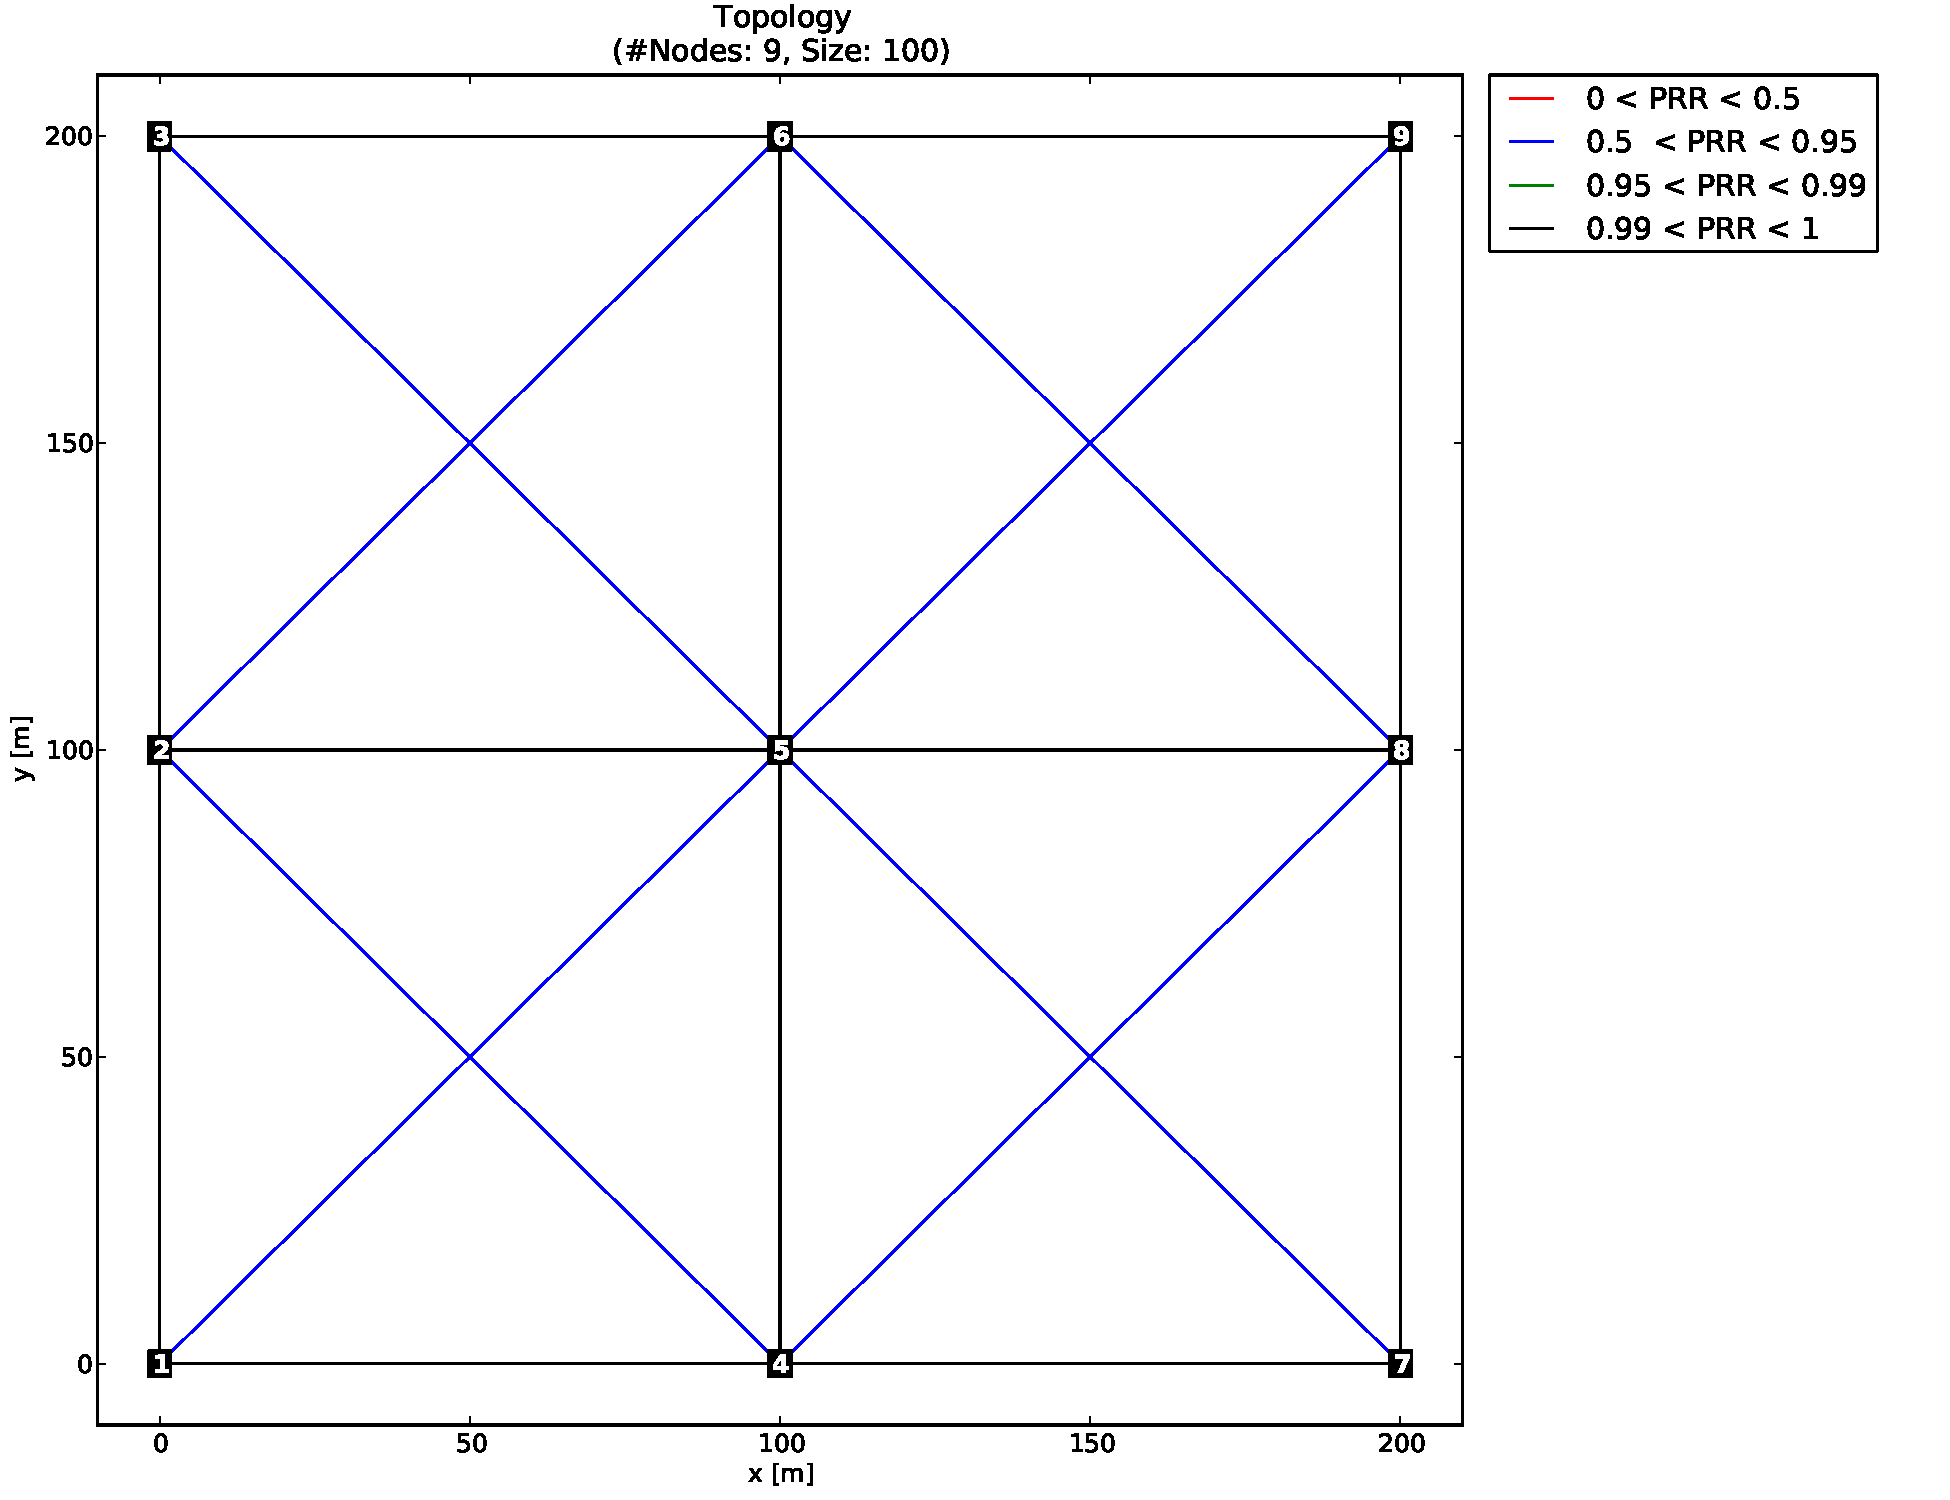
\includegraphics[scale=0.35]{Pics/results/topo9_dist100_grid.pdf}
    \caption{Grid scenario}
    \label{fig:scenario_grid}
%  \end{center}
\end{figure}

The Packet Reception Ratio (PRR) is estimated from Signal-to-Noise Ratio (SNR). The estimation is based on the measurement in~\cite{RL08}:
\[
PRR = (1-0.5*erfc(\frac{\beta_1*(SNR-\beta_2)}{\sqrt{2}}))^{46}
\quad{\beta_1} = 0.9794, {\beta_2} = 2.3851
\] 
with 
\[
SNR = Signal\:(dBm)- Noise\:(dBm) = -(50 + 20 {\log}(Distance)) - (-98)\:(dBm)
\] 
The relationship between distance and PRR is shown in Figure~\ref{fig:prr}. When the distance between two nodes is smaller than 120~m, they can hear each other with a PRR value larger than 0.99. Once the distance is larger than 120~m, the PRR begins to decline until it reaches a value of zero at a distance of 165~m.  This means that at a distance of over 165~m two nodes are at least two hops apart.

\begin{figure}[htbp]
  \begin{center}
    \leavevmode
      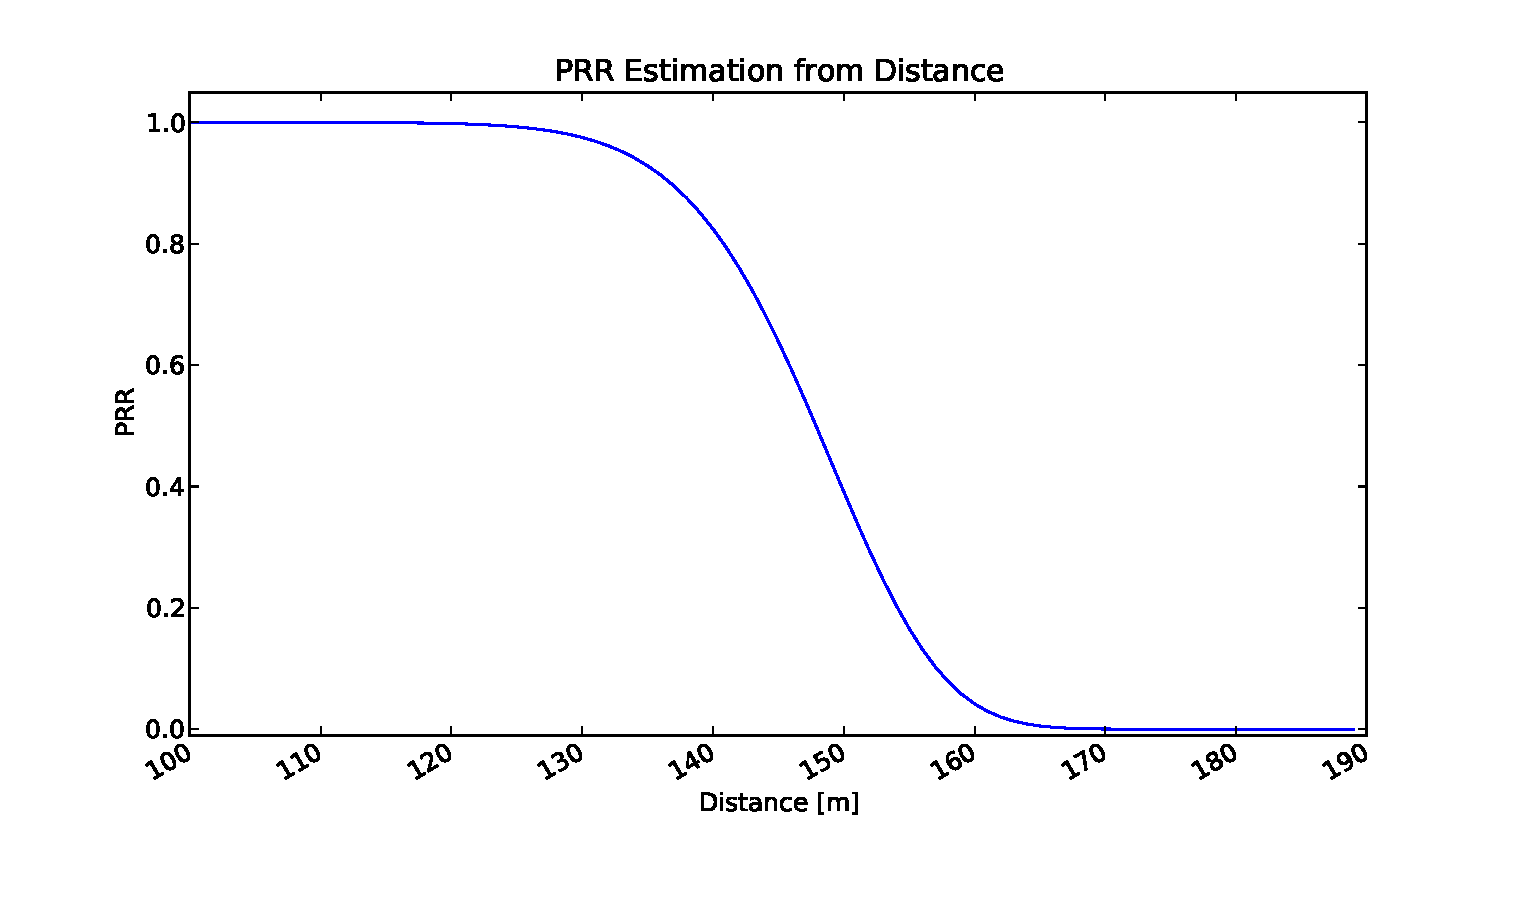
\includegraphics[scale=0.45]{Pics/prr.pdf}
   \caption{Relationship between distance and PRR}
    \label{fig:prr}
  \end{center}
\end{figure}

\subsection{Trickle Parameters and Variables}
\label{trickle parameters}
The Trickle timer parameters and initial variables of RPL in the simulation are set as below:
\begin{itemize}
\item Minimum time interval size $Imin = 256\:ms$;

\item Maximum time interval size $Imax = 262144\:ms = 256\:s$;

\item Redundancy constant $k = 255$;

\item Initial current interval size $I = 256\:ms$;

\item Initial timer value t randomly chosen in range of $[128, 256)\:ms$;

\item Initial counter $c=0$.
\end{itemize}

\subsection{Simulation Metrics}
\label{Sim:metrics}
The metrics that are used to evaluate the RPL performance are:
\begin{itemize}
\item Cumulative distribution function (CDF) of time to default route discovery: when a node receives the first DIO message from a lower rank node, it sets the default route entry. The sending of the DIO is controlled by a Trickle timer. The CDF of the default route discovery time will demonstrate the characteristics of the Trickle algorithm.

\item Mean control message overhead over 100 runs: In order to show the effect of the Trickle timer, the amount of ICMP messages a node sends out during time intervals will be shown.

\item Mean packet loss over 100 runs: Packet loss rate shows the quality of the links between nodes. A good multi-hop routing protocol should be able to forward packet properly to the destination under the certain link condition. The mean packet loss rate of both OF0 and MRHOF will be compared.

\item Mean Round-Trip Time (RTT) over 100 runs: The mean RTT for various scenarios and both OF0 and MRHOF with link ETX (hereinafter referred to as MRHOF) will be evaluated.

\end{itemize}







